%!TEX root = ../TFM.tex

\section{La Gamificación}


\coment{Esto es lo que correspondería al marco teórico.}


En esta sección procedemos a describir en términos generales la Gamificación como estrategia metodológica.
%
Primeramente trataremos de clarificar el concepto de gamificación, porqué y cómo se puede gamificar un contexto.
%
Una vez detallado, en la siguiente sección trataremos de aplicar la gamificación en la educación.


La palabra \textit{Gamificación} es una traducción del término inglés \textit{Gamification}, palabra derivada del sustantivo \textit{game}.
%
En castellano no podemos considerar Gamificación como palabra derivada de otro sustantivo. Por ello, podríamos considerar otra traducción: ludificación, palabra derivada del adjetivo lúdico.
%
Para el presente trabajo se ha preferido utilizar el término Gamificación para buscar la congruencia con la tendencia con la investigación y el profesorado.


\coment{Qué es la Gamificación}

Según \cite{GamificationDef}, la \concept[Gamificación]{gamificación} consiste en la utilización de mecánicas, estética y procesos de pensamiento de los juegos para involucrar a las personas, motivar su acción, promover el aprendizaje y resolver problemas.

Esta definición, aunque incluya la promoción del aprendizaje, no está restringida exclusivamente al ámbito educativo. 
%
De hecho, la Gamificación entendida como una estrategia o metodología es aplicada a día de hoy en diversos ámbitos. 
%
Por ejemplo, es una técnica muy utilizada en el campo del Marketing \cite{GamifyMark} y de los Recursos Humanos \cite{GamifyHR}.
%
Tanto la Educación, como los Recursos Humanos como el Marketing son contextos no lúdicos en los que podríamos utilizar elementos de juegos para involucrar a las personas, motivar su acción, promover el aprendizaje y/o resolver problemas, es decir, para gamificar.

De hecho, la consultora Gartner estudia la Gamificación y tiene su propia definición con algunos matices.
%
\cite{Gartner} define gamificación como el uso de mecánicas del juego para impulsar la participación en escenarios no lúdicos, y cambiar comportamientos en un público, con el objetivo de lograr resultados de negocio.
%
Coincide en la utilización de las mecánicas y cambiar comportamientos, sin especificar cuáles, centrándolo todo en lograr resultados de negocio.

Otra definición popular y mucho más general es la que utiliza \cite{kwerb-WhatIs}: la gamificación es la utilización de elementos de juegos en contextos no-lúdicos.

Debido a la recencia del término,

\coment{Historia de la gamificación}

Gamificación puede ser un término reciente, por ello no hay una única definición consensuada y por ello han sido presentadas diferentes definiciones.
%
Sin embargo, la idea de utilizar las mecánicas de los juegos para resolver problemas y atraer a personas no es precisamente nueva. 
%
En el entorno militar, se llevan utilizando juegos y simulaciones desde hace cientos (sino miles) de años \cite{GamificationDefII}.
%
Otra novedad, además del término y su estudio, es su gran crecimiento debido, entre otros factores a la industria del videojuego.
%


\coment{Por qué gamificar}

\paragraph{¿Por qué gamificar?} Hay bastantes investigaciones recientes que intentan contestar a esta pregunta.
%
Recurriendo a una revisión bibliográfica \cite{EmpiricalGamification} encontramos que la mayoría de experimentos empíricos sobre Gamificación han tenido efectos positivos en términos motivacionales: los participantes han participado más activamente en contextos gamificados que en contextos no gamificados.
%
Sin embargo, no todos los estudios encontraron efectos positivos en todos los participantes.
%
Además, parece que la gamificación falla a largo plazo, tal vez por el efecto de la novedad. 
%
\footnote{Estos posibles peligros y otros se tratarán más adecuadamente en \ref{PosiblesPeligros}, cuando el lector disponga de visión más global de la gamificación.}

Pero la gamificación puede producir efectos beneficiosos más allá de la motivación.
% 
De acuerdo con \cite{kwerb-WhyGamify} la Gamificación permite fidelizar a las persona, hacer todavía más social el contexto, ofrecer a la persona un sentido del progreso en ese contexto y crear un hábito.


\subsection{Diferencias entre Juegos serios y Gamificación}

Es importante distinguir gamificación de juegos serios. Los \concept[Juegos serios]{juegos serios} consisten en la modificación del contexto transformándolo en un contexto lúdico, mientras que la gamificación incorpora elementos en un contexto no lúdico, manteniendo el contexto como no lúdico.
%
Un ejemplo de juego serio sería idear un juego de conquistas como el Risk para trabajar los mapas políticos con los alumnos. 

Aunque los juegos serios tengan consecuencias positivas y puedan ser una buena herramienta\footnote{Tanto es así que \cite{MetaSerious} concluye en su revisión que los juegos serios son más efectivos en contextos de aprendizaje pero menos efectivo que los métodos convencionales en términos motivacionales.}, su estudio se sale de esta tesis.

\subsection{Aspectos de la Gamificación}

\paragraph{Diseño enfocado en la persona:} 
Un contexto gamificado crea una experiencia.
%
De acuerdo con el ganador del premio \textit{Gamification Guru of the year 2016}\footnote{Premio otorgado en el congreso europeo más grande de Gamificación a nivel internacional, el World Gamification Congress (WCW - Barcelona).}, \cite{BeyondPBL}, la gamificación se diseña enfocada en la persona en contraposición con el diseño enfocado en la función o el resultado.
%
La situación se transforma en una experiencia para el usuario, y esta es una de las claves.

Aunque pueda ser una obviedad, en un juego hay jugadores. 
%
No son tratados como participantes ni como usuarios, sino como jugadores.
%
Pensar en las personas participantes de un contexto que se quiere gamificar como jugadores es el primer paso para realizar un diseño enfocado en la persona.
%
Sitúa a esas personas como los protagonistas y como el centro de la experiencia, pues para eso están diseñados los juegos.
%
Además, los jugadores tienen un cierto sentido de autonomía y control sobre la experiencia.

Otra clave a considerar es la siguiente: un juego tiene la meta de que sus jugadores empiecen a jugar, frente a otras posibilidades a su alcance, y se mantengan jugando.
%
Una manera de conseguir esta meta es hacer el recorrido del juego o la experiencia gamificada con una dificultad que se incremente progresivamente y de acuerdo a lo que el jugador puede conseguir en cada momento. 
%
Según el profesor Werbach, es importante que al principio del recorrido sea imposible fracasar, para lo que será necesario diseñar guías y limitar las posibilidades existentes e ir desbloqueándolas a medida que el jugador avanza en la experiencia.


\paragraph{La anatomía de la diversión: }

Una herramienta muy importante mediante la cual los juegos consiguen las claves mencionadas anteriormente es mediante la diversión.
%
Es impensable un juego que sea aburrido de jugar.
%
De la misma manera, una gamificación tiene que ser divertida.
%
Es importante esclarecer que hay varios tipos de diversión.
%
De acuerdo con \cite{whyweplaygames} hay 4 tipos de diversión: 
%
\concept[Diversión\IS Fácil]{Diversión fácil} -- aquella diversión que se produce ante un disfrute de la experiencia, manteniendo la atención del jugador. Se basa en la curiosidad y la intriga --;
%
\label{kindsoffun}
\concept[Diversión\IS Difícil]{Diversión difícil}  -- aquella diversión que producen los retos que requieren habilidad y estrategia más que suerte y que permiten al jugador constatar cuan bueno es--;
%
\concept[Diversión\IS Social]{Diversión social} -- aquella diversión que se fundamenta en la relación con otras personas durante el juego --;
%
\concept[Diversión\IS Interna]{Diversión interna} -- aquella diversión producida por las experiencias internas como el alivio, el entusiasmo y la agitación.

Esta no es la única clasificación de la diversión.
%
En \cite{MDA} encontramos una división en 8 tipos: sensación, fantasía, narrativa, retos, social, descubrimiento, expresión, pasatiempo.
%
\label{AnatomyOfFun}
%

Esta anatomía de la diversión es fundamental para diseñar una buena gamificación.
%
Un entorno laboral o un contexto educativo normalmente no se caracterizan por ser intrínsecamente divertidos.
%
¿Podemos enfocar la gamificación para trabajar o aprender desde alguna de las dimensiones de la diversión? 
%
El potencial de la diversión difícil es inmenso. 
%
De hecho, algunas personas buscan que su trabajo sea un reto continuo.
%
Por otro lado, ¿cuántos estudiantes van a los centros educativos porque van sus amigos?
%
Y eso podría considerarse que la dimensión social les divierte.


\paragraph{Teoría del Flujo:} La teoría de Csikszentmihalyi investiga e intenta responder a la situación en la que una persona está tan inmersa en una actividad que se olvida de otras circunstancias como el cansancio, el hambre o la incomodidad.
%
A este estado lo llamó \textit{flow}, que en el campo de la Psicología hispanohablante se traduce por \concept[Flujo]{flujo}.
%
Este estado se produce en actividades autotélicas \label{autotel}, es decir, en actividades cuyo fin es la realización de la propia actividad.
%
Las condiciones del flujo incluyen que la percepción de desafío de la tarea y de habilidad sean similares y elevadas, que estén claras las metas intermedias y que se reciba feedback inmediato sobre el progreso\cite{Flow}.
%
En la figura \ref{fig::Flujo} se resumen los posibles estados dependiendo del balance entre el nivel de desafío y la habilidad.

\begin{figure}[hbt]
\begin{center}
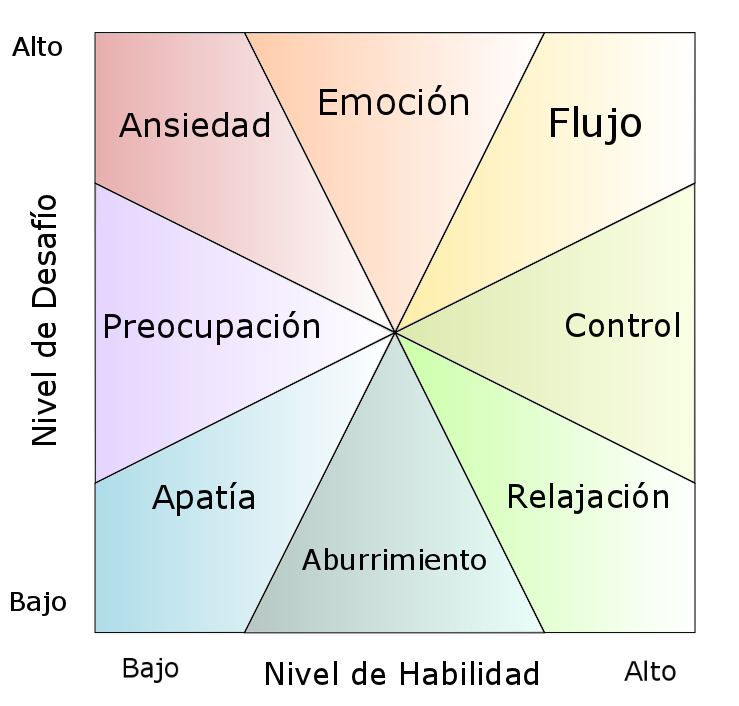
\includegraphics[scale=0.40]{img/Flujo.png}
\caption{Estados de la teoría del flujo.}
\label{fig::Flujo}
\small{Fuente: http://www.cluehuntervalencia.com}
\end{center}
\vspace{-0.5cm}
\end{figure}
\FloatBarrier

Csikszentmihalyi entrevistó a jugadores de ajedrez, artistas y deportistas, pero hoy en día, este fenómeno se produce con mucha frecuencia entre los gamers\footnote{Personas con una gran afición por los videojuegos}.
%
La distorsión de la percepción temporal que se produce en el estado de flujo es muy habitual.
%
¿Es posible establecer las condiciones necesarias en un sistema gamificado para que los jugadores entren en estado de flujo?


\subsection{Elementos de la Gamificación}

En esta sección vamos a ver los elementos y las herramientas generales con las que una persona puede diseñar una gamificación para un contexto específico.

Los elementos de la Gamificación son los elementos que podemos encontrar en los juegos, atendiendo a \cite{werbach2012win} son: dinámicas, mecánicas y componentes, de mayor a menor abstracción.

\concept{Dinámicas} 
%
Las dinámicas son las estructuras implícitas del juego. 
%
Por ejemplo, las reglas serían una manifestación superficial de esa estructura implícita, pero las dinámicas también incluirían manifestaciones conceptuales como podrían ser las restricciones básicas de los juegos, por ejemplo, el respeto a las normas.
%
Por ejemplo, se considerarían dinámicas también las emociones, la narrativa, la progresión y las relaciones personales.\todo{¿Debería incluir alguna definición de los componentes concretos?} 

\concept{Mecánicas} Las mecánicas son los procesos que definen formalmente el contexto y que hacen avanzar la acción. 
%
Por ejemplo se considerarían mecánicas los retos, la suerte, la competición y la cooperación, el feedback, las recompensas, la adquisición de recursos, las transacciones y los estados de finalización.

\concept{Componentes} Los componentes son las instancias específicas de mecánicas y dinámicas. 
%
Serían componentes los logros, los avatares, los jefes finales\footnote{Batalla muy difícil que tiene lugar al final de cada nivel.}, los combates, el desbloqueo de contenido, los niveles, las misiones, los equipos, las posesiones y el grafo social 
%
Además, hay 3 componentes que merecen una mención específica: los puntos (points), las medallas (bdages) y las clasificaciones (leaderboards), comúnmente llamados \gls{PBL}.


\paragraph{La gamificación es más que \gls{PBL}:} Es habitual confundir gamificación con un sistema de recompensas basado en \gls{PBL}. 
%
La gamificación trata de crear una experiencia centrada en el jugador. 
%
La implementación de un sistema de recompensas enfocado a realizar con eficiencia la función, dejando de lado la experiencia de los jugadores no puede ser considerada una gamificación y de hecho puede ser contraproducente.

Esta confusión es habitual porque estos tres componentes son fáciles de implementar y tienen varias funciones específicas que resultan muy útiles.
%
Los \textbf{puntos}, por ejemplo, otorgan un feedback acerca del rendimiento y el progreso, es una fuente de datos importante para el diseñador, pueden ligarse con recompensas y se pueden utilizar para determinar los estados de finalización.
%
Las \textbf{medallas} tienen una flexibilidad que permite definir el estilo de un jugador. 
%
Además, tienen un componente social muy importante, ya que muestran el estatus del jugador y son una representación de los logros conseguidos. 
%
También, algunos jugadores se sienten motivados a coleccionarlas.
%
Por último, las \textbf{clasificaciones} o leaderboards crean un cierto sentido de competición, en el que los jugadores quieren ascender a puestos más altos de la clasificación, podría ser por el estatus que ofrecen esas posiciones.
%
Se ha estudiado que los leaderboards completos desmotivan al 80\% de las personas, debido a la gran brecha que se produce entre los primeros puestos y los últimos.
%
La aproximación más utilizada es diseñar leaderboards entre grupos más pequeños de jugadores, por ejemplo, entre los jugadores más cercanos con una puntuación cercana o con sus amigos.


\subsubsection{Teoría de la motivación}
\label{SDT}
\label{PosiblesPeligros}
En la Psicología de la Motivación se ha establecido una diferencia entre 2 tipos de motivaciones \cite{SDT}:  \concept[Motivación\IS Intrínseca]{Motivación intrínseca} -- aquella que depende de los procesos cognitivos internos y está dirigida por el sentido de la autocompetencia, autonomía y relación -- y la \concept[Motivación\IS Extrínseca]{motivación extrínseca} -- aquella que depende de las recompensas que se puedan adquirir con la conducta realizada.
%
Por ejemplo, las actividades autotélicas, mencionadas en la teoría de flujo (ver \ref{autotel}), necesariamente conllevan una motivación intrínseca.
%
Además de esta diferencia se ha constatado que las conductas motivadas extrínsecamente, sobretodo motivadas con recompensas tangibles aunque también ocurre con las recompensas verbales, dejan de realizarse cuando desaparece la fuente de motivación, incluso cuando en un momento anterior a la aparición de recompensas la conducta se llevara a cabo motivada intrínsecamente
%
\cite{ExtrinsicEatsIntrinsic}.

La motivación intrínseca se basa en la \textit{autonomía}, tener la situación bajo control y poder determinar el resultado de las acciones; \textit{competencia} como necesidad de saberse capaz y competente ante los retos y dificultades y \textit{pertenencia} a algo más grande que la propia persona: conectar con otras personas, sentirse parte de la sociedad y compartir los logros.


Es importante conocer esta diferencia a la hora de plantear el objetivo de nuestra gamificación. 
%
Es más sencillo diseñar un sistema de refuerzos basado en el condicionamiento operante, puramente extrínseco que diseñar un sistema que alimente los deseos de autonomía, competencia y pertenencia para fomentar fomentar la motivación intrínseca.
%
¿Interesa al diseñador crear un sistema sencillo basado en la motivación extrínseca de los jugadores o, por el contrario, diseñar un sistema más complejo que fomente y haga crecer la motivación intrínseca?


\subsubsection{Taxonomía de los jugadores}

\index{Taxonomía de\IS Bartler}
%
En el proceso de investigación sobre los juegos, sus motivaciones e impactos se ha constatado que no todas las personas responden igual a todos los juegos porque hay tipos de jugadores. 
%
Habiendo distintos tipos de jugadores, no todas las personas responderán por igual a los mismos elementos del juego y habrá elementos más afines a unos tipos de jugadores que a otros.

Vamos a estudiar algunas teorías que han tratado de definir una taxonomía de los jugadores, es decir, de clasificar los tipos de jugadores.

\cite{TypeMUD} estudia a los jugadores de \gls{MUD} según su personalidad y los comportamientos mostrados, según 2 variables: centrados en los jugadores o en el mundo, centrados en la acción y los objetivos del juego o en la interacción entre jugadores.
%
Estas 2 variables dan lugar a 4 tipos de jugadores, resumido en la imagen \ref{fig::Bartle}:
\begin{itemize}
	\item  \textbf{Triunfadores} (\textit{achievers}): centrados en la acción y en el mundo.
	%
	Tienen un comportamiento individual y quieren llegar a ser los primeros rápidamente.
	

	\item \textbf{Ambiciosos} (\textit{killers}): centrados en la acción y en los jugadores. 
	%
	Estos jugadores buscan las primeras posiciones y además, que los otros jugadores pierdan (de ahí que estén centrados en los jugadores).
	

	\item \textbf{Exploradores} (\textit{explorers}): centrados en la interacción y en el mundo.
	%
	Quieren descubrir y aprender aspectos nuevos del sistema.

	\item \textbf{Sociables} (\textit{socializers}): centrados en la interacción y en los jugadores.
	%
	Juegan para relacionarse con otros jugadores, compartir ideas y experiencias.
\end{itemize}

Se han desarrollado algunos test para clasificar a un jugador en concreto en base a un cuestionario \cite{Bartletest}.
%
En esta taxonomía no se establece la pertenencia a un tipo único, es decir, una persona puede ser 80\% ambicioso, 15\% triunfador y 5\% explorador.


\begin{figure}[hbt]
\begin{center}
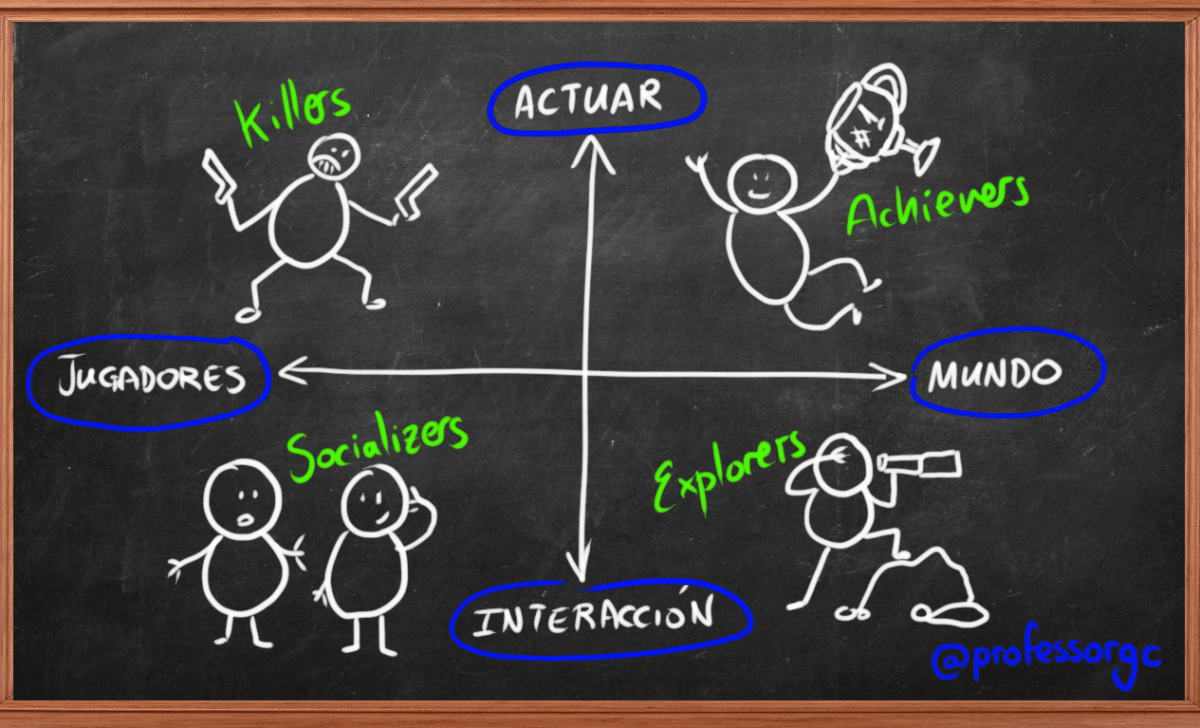
\includegraphics[scale=0.25]{img/Bartle.png}
\caption{Taxonomía de los jugadores según Bartle.}
\label{fig::Bartle}
\vspace{-0.25cm}
\small{Fuente: \url{Creatividadenblanco.com}.}
\end{center}
\end{figure}

Esta clasificación presenta ciertas limitaciones. 
%
La más importante es que se centra en videojuegos \gls{MUD} y, por lo tanto, no es extrapolable a otros juegos; mucho menos a contextos gamificados.
%
Además, el término \textit{killers} en contextos diferentes de videojuegos \gls{MUD} no parece muy adecuado.


\index{Taxonomía de\IS Amy Jo Kim}
%
Por ello, podemos recurrir a la teoría de \cite{AmyJoKim}, que se basa en la de Bartle pero la modifica para superar esa limitación.
%
Defien también 4 tipos de jugadores denominados con verbos principales que describen su guía de acción y otros verbos secundarios, como se puede ver en la imagen \ref{fig::AmyJoKim}.
%
La clasificación la hace en base a 2 variables: centrados en el contenido o centrados en los jugadores y centrados en actuar o en interactuar.
%
Los jugadores centrados en el contenido y en la actuación serían los competidores (\textbf{compete}), buscando la superación personal.
%
Quienes se centran en el contenido y en la interacción serían los exploradores (\textbf{explore}), buscando el acceso al conocimiento y la información.
%
Los que se centran en los jugadores y en la actuación serían los colaboradores (\textbf{collabore}), buscando formar parte de algo más grande para poder ganar juntos.
%
Por último, las personas que se centran en los jugadores y en la interacción serían los expresivos (\textbf{express}), buscando manifestarse y mostrar su creatividad.

\begin{figure}[hbt]
\begin{center}
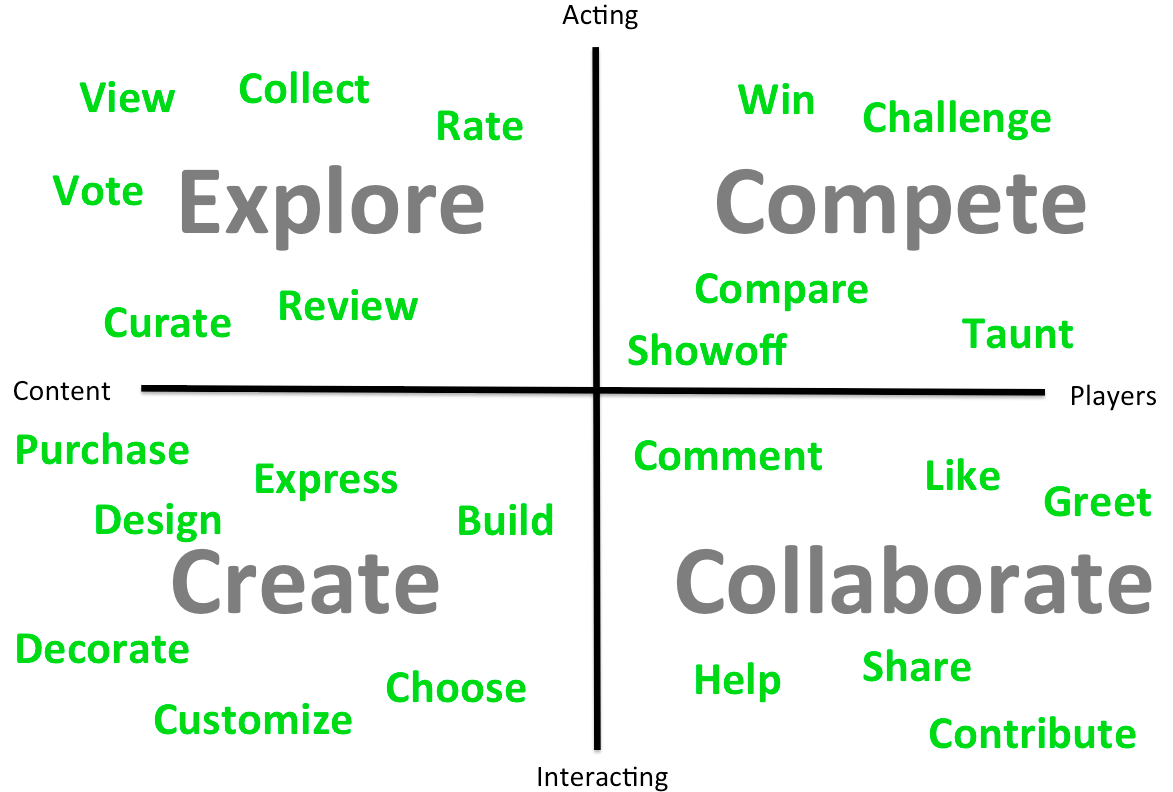
\includegraphics[scale=0.25]{img/AmyJoKim.png}
\caption{Taxonomía de los jugadores según Amy Jo Kim.}
\label{fig::AmyJoKim}
\vspace{-0.25cm}
\small{Fuente: \url{http://amyjokim.com}.}
\end{center}
\end{figure}


La teoría de Marczewski \cite{marczewski} es más amplia que las anteriores.
%
Establece más tipos de jugadores, pero además distingue entre jugadores motivados intrínsecamente y extrínsecamente.
%
No sólo eso, sino que los tipos de jugadores motivados extrínsecamente tienen a su vez subgrupos que se parecen a los motivados intrínsecamente, de tal manera que es posible convertir a un jugador motivado extrínsecamente en un jugador motivado intrínsecamente.

En la figura \ref{fig::Marczewski} se puede apreciar el correspondiente esquema de la teoría.
%
En el centro, encontramos el motivo que guía a cada tipo de jugador. 
%
De estos motivos 4, según \cite{marczewski} son intrínsecos (Autonomía, Maestría, Relaciones, Propósito\footnote{El único nuevo respecto a la teoría de la auto-determinación \cite{SDT} es el motivo de \textit{propósito}}) y 2 son extrínsecos: cambio y recompensas.
%
En base a estos 6 motivos, se establecen los 6 tipos de jugadores:
%
\begin{itemize}
	\item \textbf{Espíritus libres} (\textit{Free spirit}): están motivados por la autonomía. Buscan crear y expresarse.

	\item \textbf{Triunfadores} (\textit{Achiever}): están motivados por la maestría. 
	%
	Buscan aprender cosas nuevas, mejorar y retos que superar.


	\item \textbf{Socializadores} (\textit{Socialiser}): motivados por las relaciones.
	%
	Buscan interactuar con los demás y crear conexiones sociales.

	\item \textbf{Filántropos} (\textit{Philantropist}): movidos por el motivo de propósito y significado.
	%
	Buscan conseguir un propósito que tenga  significado para ellos.
	%
	Son altruistas y están dispuestos a ayudar a otras personas.


	\item \textbf{Jugadores} (\textit{Player}): están motivados por las recompensas. 
	%
	Harán lo que haga falta para conseguir las recompensas del sistema.
	\subitem Este tipo de jugador también tiene 4 subgrupos: egoísta (self-esteemer), consumidor (consumer), contacto (networker), explotador (exploitationer).

	\item \textbf{Perturbador} (\textit{Disruptor}): les motiva el cambio. En general buscan interrumpir el sistema de forma directa o indirectamente (a través de otros usuarios) para forzar el cambio positivo o negativo.
	\subitem Este tipo de jugador, motivado extrínsecamente tiene 4 subgrupos: influenciador (influencer), destructor (destroyer), mejorador (improver), duelistas (griefer).
\end{itemize}

\begin{figure}[hbtp]
\begin{center}
\index{Taxonomía de\IS Marczewski}
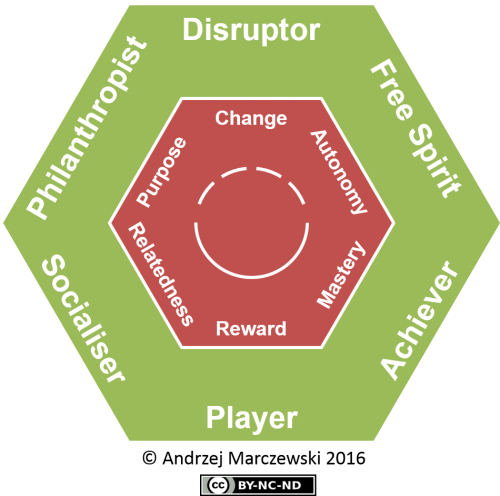
\includegraphics[scale=0.65]{img/Marczewski.jpg}
\caption{Taxonomía de los jugadores según Marczewski.}
\label{fig::Marczewski}
\vspace{-0.25cm}
\small{Fuente: \url{http://elearningindustry.com}.}
\end{center}
\end{figure}
\FloatBarrier

Como decíamos, esta teoría ofrece un marco de actuación para modificar las motivaciones de los jugadores y transformar a los jugadores extrínsecamente motivados en intrínsecamente motivados.
%
En la figura \ref{fig::MarczewskiEvol} se resume la propuesta de \cite{marczewski} sobre una posible ruta de evolución de los jugadores para la que, según él, hay cierta evidencia.

\begin{figure}[hbtp]
\begin{center}
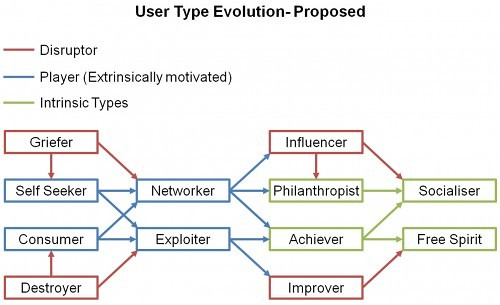
\includegraphics[scale=0.65]{img/evolution.jpg}
\caption{Posible conversión de los jugadores según la taxonomía de Marczewski.}
\label{fig::MarczewskiEvol}
\vspace{-0.25cm}
\small{Fuente: \url{http://gamified.uk}.}
\end{center}
\end{figure}
\FloatBarrier



\subsubsection{Impacto de la competición en la motivación}


La competición es otra herramienta más a disposición del diseñador, pero es importante tener claro el resultado de algunas investigaciones.
%
Por ejempo, \cite{Crawford_CompetitionDef} señala que la competición puede centrar la atención en impedir que el contrincante venza en lugar de centrarse en mejorar y optimizar su propio desempeño.

Otro fenómeno estudiado por \cite{n-effect} es que el número de competidores y la motivación de los mismos mantienen una relación inversamente proporcional, es decir, cuantos más competidores, menor motivación.

Por último, un estudio llevado a cabo sobre la competición en la educación \cite{CompetitionInEd} constata que los premios para los ganadores deberían ser de poca importancia o incluso simbólicos para asegurar que el esfuerzo de los estudiantes es intrínseco y no está dirigido por la expetativa del premio.


\section{Educación gamificada}

Hasta ahora hemos estado tratando la Gamificación en términos generales, sin centrarnos específicamente en la educación. 
%
En esta sección trataremos de estudiar cómo se adapta esa teoría general al ecosistema de un aula.


\coment{Porqué gamificar la educación}

\cite{lee2011gamification} sugieren que el sistema educativo ya contiene elementos de la gamificación, más concretamente \gls{PBL}, ya que los estudiantes realizan unos exámenes para obtener una calificación (puntos) y si se han obtenido más de 5 puntos, se obtiene la medalla de \textit{aprobado}.
%
Incluso, se puede obtener la medalla de \textit{mención de honor} en la evaluación final.
%
Además, encubiertamente se forma un leaderboard, ya que los alumnos tienen claro quienes son los mejores y los peores alumnos (en términos de calificaciones obtenidas).
%
Sin embargo, estos elementos no implican necesariamente motivación por parte de los alumnos.
%
Diseñar una gamificación en un aula puede motivar a los estudiantes, ofrecer a los profesores mejores herramientas para guiar y recompensar a sus estudiantes y enseñar a los estudiantes que la educación puede ser una experiencia divertida \cite{lee2011gamification}.

Es importante tener en cuenta la teoría de la auto-determinación (ver \ref{SDT}) y diseñar una gamificación en el contexto educativo que no debe basarse en una motivación extrínseca, sino fomentar la motivación intrínseca. 
%
De esta manera, los estudiantes podrán desarrollar una mayor capacidad para valorar el aprendizaje y cuando avancen a lo largo del sistema educativo sean capaces de aprovechar contextos educativos no gamificados. 


En la sección \ref{sec:EstadoEducacionMates} se comentó la existencia de un círculo vicioso (ver figura \ref{fig::circuloVicioso}) y que la variable más influyente en el rechazo hacia las Matemáticas en España es la percepción de la materia como aburrida o divertida.
%
Esperamos que, tras lo expuesto, el lector esté de acuerdo en que la Gamificación puede ayudar a modificar esa percepción aprovechando que existen tareas difíciles y divertidas (ver \ref{kindsoffun}) además de romper el círculo vicioso por 2 extremos diametralmente opuestos: aburrimiento y desmotivación.

\coment{¿Se puede gamificar la educación? Sí, Cook. 2013}


\subsection{Proceso de diseño de a Gamificación}

Para diseñar una buena gamificación es necesario seguir un proceso y hay quienes han propuesto un marco con unas pautas para seguir en la tarea. 
%
Como no hay un método consensuado presentaremos 2: uno más general (\cite{werbach2012win}) y otro más aplicado al contexto educativo \cite{kapp2013gamification}.

Werbach define 6 pasos para diseñar una buena gamificación con 6 D's: 
1 - Definir los objetivos de negocio; 2 - Delinear los comportamientos deseados; 3 - Describir a los jugadores; 4 - Diseñar los bucles de actividades; 5 - No olvidarse de la diversión (en inglés: \textit{Don't forget the fun}); 6 - Implementar las herramientas apropiadas (en inglés: \textit{Deploy}).
%
Esta propuesta es demasiado general y no tiene en cuenta algunas características fundamentales del contexto educativo, por ejemplo, la necesidad de un sistema de evaluación.
%
Por ello, una propuesta más centrada en el ámbito educativo puede resultar más útil, sin ignorar por completo la propuesta de Werbach.

La otra propuesta, \cite{kapp2013gamification}, tiene algunos elementos en común con la de Werbach, pero otros diferentes. 
%
Los autores estableces que se debe pasar por cuatro fases en la gamificación de un contexto educativo. 1 - Responder a las preguntas base; 2 - Responder a las preguntas de práctica; 3 - Diseñar el sistema de valoración y clasificación; 4 - Jugar al juego.

Las preguntas base hacen referencia a 5 aspectos: identificar el problema, estudiar los comportamientos existentes, definir los comportamientos deseados, tener claro el objetivo competencial (competencias que los estudiantes necesitan adquirir para que consideremos éxitosa la gamificación) y valorar aspectos que pueden mostrarnos que los alumnos están aprendiendo.
%
Por otro lado, las preguntas de práctica son las preguntas sobre el público objetivo de la gamificación (edad, conocimientos previos, habilidades, tipos de jugadores, etc.) , la logística (lugar, momento, tiempo invertido y dinámicas, mecánicas y componentes a utilizar) y las cuestiones técnicas (la utilización de herramientas TIC o no, tanto en el contexto escolar como en el contexto familiar de los estudiantes).
%
En cuanto al sistema de valoración y clasificación es necesario un arduo trabajo.
%
La base logística del sistema tiene que ser completa, es decir, no puede darse el caso en el que no esté especificada la obtención o no de una recompensa o la siguiente meta a alcanzar.
%
Este aspecto es importante, ya que puede haber jugadores que se dediquen a buscar fallos en el sistema y a romperlo para ganar.
%
Por ejemplo, los jugadores de tipo perturbador, según la teoría de \cite{marczewski}, más concretamente los duelistas dentro de los perturbadores podrían romper la gamificación si encontraran una incompletitud o inconsistencia en el sistema evaluativo.
%
Además, es necesario que el sistema sea justo y permita obtener calificaciones acordes con las competencias y habilidades adquiridas, por ello, las actividades del proyecto, la valoración y el resultado final deben ir unidos.
%
Por último, hay que saber qué acciones pueden realizar los jugadores cuando interactúen (distribuir recursos, coleccionar, cooperar, realizar misiones por otros jugadores, reintentar tareas, etc.). 
%
Es necesario también definir los estados ganadores y el número de oportunidades en cada actividad.

Durante la implementación de la gamificación es importante no perder de vista uno de los puntos que incluye Werbach: No olvidar la diversión.
%
Si un aula gamificada no es divertida para los estudiantes necesitamos revisar su diseño y reoformarla.
%
El comienzo del siguiente capítulo tendrá como marco de referencia los pasos que acabamos de tratar para guiar el proceso de diseño de la gamificación para un aula de Matemáticas en la Educación Secundaria del sistema educativo español.


